\section{Probability and impact matrix}
Beyond the definitions of probability and impact, a further quantitative analysis of risk is required. Every risk is assigned a rate based on its probability and impact scores. According to the rate, the risks are classified by their importance: the higher the risk rating, the higher their priority for attention.

To manage ratings in a more organized manner, the probability and impact matrix is defined. This matrix specifies combinations of probability and impact that lead to rating the risks as very low, low, moderate, high or extreme. The following tables show the risk rating legend used for the elaboration of this project risk matrix:
\begin{table}[H]
\centering
\begin{tabular}{c}
	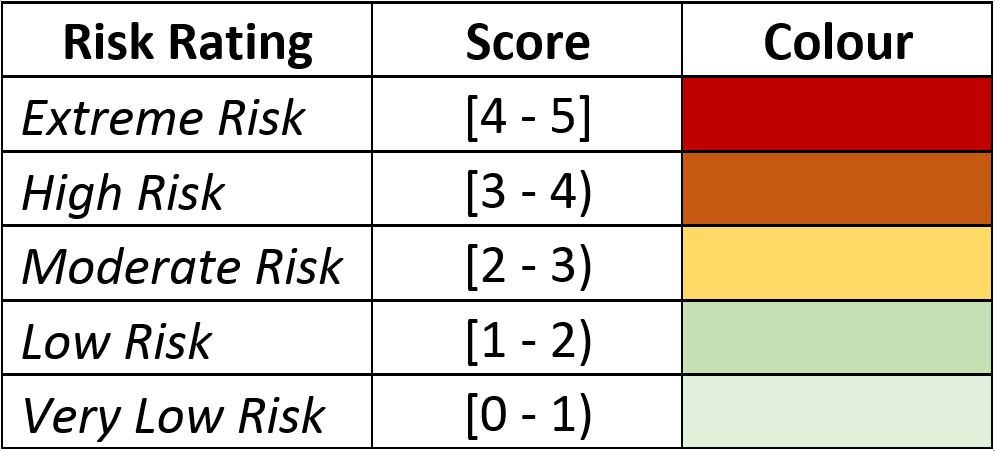
\includegraphics[width=0.5\textwidth]{./images/RiskRating}
\end{tabular}
\caption{Risk Rating Legend}
\end{table}
\begin{table}[H]
	\centering
	\begin{tabular}{c}
	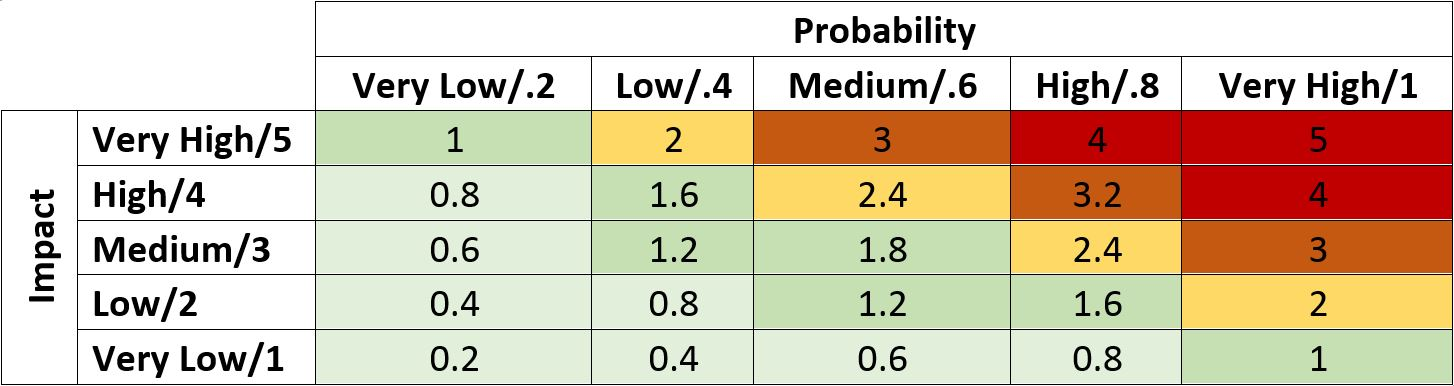
\includegraphics[width=\textwidth]{./images/Probability_and_impact_matrix}
	\end{tabular}
	\caption{Probability and Impact Matrix}
\end{table}
Depending on the risk score, the response and priority assigned to a risk will change. For example, risks that are in the red area of the matrix (high probability and high impact) may require priority action and aggressive response strategies while risks in the light green area may not require proactive management action beyond being considered as a warning.
Throughout the project risks may vary so, using this matrix, risks will be reconsidered, changing their rating if necessary.
